\documentclass{article}

\title{\vspace{-5mm}%
	\fontsize{24pt}{10pt}\selectfont
	\textbf{Formelsammlung}
}
\usepackage{pgfplots}


\usepackage{enumitem}
\usepackage[utf8]{inputenc}
\usepackage{amsmath}

\begin{document}
\maketitle	
\pagebreak

\tableofcontents
\pagebreak


\section{Bayes’scher Ansatz}

\subsection{Entscheidungsregionen}
Bei gleicher Klassifizierungswahrscheinlichkeit gilt


$$p(x|C_1) = p(x|C_2)$$

$$ p(x|C_i) = \frac{1}{\sqrt{2\pi \sigma^{2}_i}} \cdot e^{\frac{-\frac{1}{2}(x-\mu_i)^2}{\sigma_{i}^2}}$$

\subsubsection{Ungleiche Klassifizierungswahrscheinlichkeit}
Wenn eine Klasse wahrscheinlicher ist so gilt

$$p(C_1) \cdot p(x|C_1) = p(x|C_2) \cdot p(C_2)$$


$$ \frac{p(C_1)}{p(C_2)} \cdot \frac{\sqrt{2\pi \sigma^{2}_2}}{\sqrt{2\pi \sigma^{2}_1}} = e^{\frac{-\frac{1}{2}(x-\mu_2)^2}{\sigma_{2}^2} - \frac{-\frac{1}{2}(x-\mu_1)^2}{\sigma_{1}^2}} $$
$\frac{p(C_1)}{p(C_2)}$ definieren wir als $\mathcal{P}$. Als Reziproge von $\mathcal{P}$ bezeichnen wir$\mathcal{P}'$. Bei gleichen Wahrscheinlichkeiten $ p(C_{1/2}) = 0,5$ ist $\mathcal{P} = 1$ und kann ignoriert werden.

\subsubsection{Fehlklassifizierung}

Wenn eine Verlustmatrix $V$ gegeben ist so wird die Gewichtung der Fehlklassifikation pro Klasse berücksichtigt über 

$$V_{1,2} \cdot p(x|C_1) = p(x|C_2) \cdot V_{2,1}$$

$$ \frac{V_{1,2}}{V_{2,1}} \cdot \frac{\sqrt{2\pi \sigma^{2}_2}}{\sqrt{2\pi \sigma^{2}_1}} = e^{\frac{-\frac{1}{2}(x-\mu_2)^2}{\sigma_{2}^2} - \frac{-\frac{1}{2}(x-\mu_1)^2}{\sigma_{1}^2}} $$
$\frac{V_{1,2}}{V_{2,1}}$ definieren wir als $\mathcal{V}$. Bei gleicher Verlustgewichtung $ V_{(1/2),(2/1)} = x$ ist $\mathcal{V} = 1$ und kann ignoriert werden.

\subsubsection{Umformung}
Mit diesen Parametern kann die Formel wie folgt umgeformt werden

\begin{equation} \label{trans:1}
ln(\mathcal{P} \cdot \mathcal{V} \cdot \frac{\sqrt{\sigma^{2}_2}}{\sqrt{\sigma^{2}_1}}) = \frac{-\frac{1}{2}(x-\mu_2)^2}{\sigma_{2}^2} - \frac{-\frac{1}{2}(x-\mu_1)^2}{\sigma_{1}^2}
\end{equation}

\begin{align}
\sigma_{2}^2 \cdot \sigma_{1}^2 \cdot ln(\mathcal{P} \cdot \mathcal{V} \cdot \frac{\sqrt{\sigma^{2}_2}}{\sqrt{\sigma^{2}_1}}) &= -\frac{1}{2} \cdot \sigma_{1}^2 (x-\mu_2)^2 - -\frac{1}{2} \cdot \sigma_{2}^2 (x-\mu_1)^2
%  -2 \cdot \sigma_{2}^2 \cdot \sigma_{1}^2 \cdot ln(\mathcal{P} \cdot \mathcal{V} \cdot \frac{\sqrt{\sigma^{2}_2}}{\sqrt{\sigma^{2}_1}}) = 
\\
&=
\sigma_{1}^2 (x^2 - 2\mu_{2}x + \mu_{2}^2) - 
\sigma_{2}^2 (x^2- 2\mu_{1}x + \mu_{1}^2) 
%  -2 \cdot \sigma_{2}^2 \cdot \sigma_{1}^2 \cdot ln(\mathcal{P} \cdot \mathcal{V} \cdot \frac{\sqrt{\sigma^{2}_2}}{\sqrt{\sigma^{2}_1}}) 
\\
& = 
(\sigma_{1}^2 - \sigma_{2}^2) \cdot x^2 +
(-\mu_{2}\sigma_{1}^2 + \mu_{1} \sigma_{2}^2)2x 
+ \sigma_{1}^2 \mu_{2}^2 - \sigma_{2}^2\mu_{1}^2
\end{align}


\begin{equation}
\begin{aligned}
0 = 
(\sigma_{1}^2 - \sigma_{2}^2) \cdot x^2 +
(-\mu_{2}\sigma_{1}^2 + \mu_{1} \sigma_{2}^2)2x 
+ \sigma_{1}^2 \mu_{2}^2 - \sigma_{2}^2\mu_{1}^2
+ 2 \cdot \sigma_{2}^2 \cdot \sigma_{1}^2 \cdot ln(\mathcal{P} \cdot \mathcal{V} \cdot \frac{\sqrt{\sigma^{2}_2}}{\sqrt{\sigma^{2}_1}})
\end{aligned}
\end{equation}

\subsubsection{pq-Formel}
Benötigt einen Ausdruck der Form $x^2 + px +q = 0$.
Um die pq-Formel $x_{1/2} = - \frac{p}{2} \pm \sqrt{(\frac{p}{2})^2-q}$ anzuwenden muss der Term mit $/ \div (\sigma_{1}^2 - \sigma_{2}^2)$ umgeformt werden

\subsection{Zurückweisung}
$$p(C_1 | x) \ge \theta $$

$$ p(C_1 | x) = \frac{p(C_1) \cdot p(x| C_1)}{p(x)}$$

$$p(x) = p(C_1) \cdot p(x | C_1) + p(C_2) \cdotp(x| C_2) $$

$$ \frac{p(C_1) \cdot p(x| C_1)}{p(C_1) \cdot p(x | C_1) + p(C_2) \cdotp(x| C_2)} \ge \theta$$
Dieser Ausdruck hat die Form $\frac{A}{A+B}$ was umgeformt werden kann in $\frac{1}{1+\frac{B}{A}}$


$$ \frac{1}{1+\frac{p(C_2) \cdotp(x| C_2)}{p(C_1) \cdot p(x| C_1)}} \ge \theta$$
\begin{align}
1 &\ge \theta (1+\frac{p(C_2) \cdotp(x| C_2)}{p(C_1) \cdot p(x| C_1)}) 
\\
\frac{1}{\theta} &\ge 1+ \mathcal{P}' \cdot \frac{p(x| C_2)}{ p(x| C_1)}
\\
 \frac{1}{\theta} - 1 &\ge
\mathcal{P}' \cdot \frac{\frac{1}{\sqrt{2\pi \sigma^{2}_2}} \cdot e^{\frac{-\frac{1}{2}(x-\mu_2)^2}{\sigma_{2}^2}}}{\frac{1}{\sqrt{2\pi \sigma^{2}_1}} \cdot e^{\frac{-\frac{1}{2}(x-\mu_1)^2}{\sigma_{1}^2}}} 
\\
  \frac{1}{\theta} - 1 &\ge 
\mathcal{P}' \cdot
\frac{\sqrt{2\pi \sigma^{2}_1}}{\sqrt{2\pi \sigma^{2}_2}}
 \cdot e^{\frac{-\frac{1}{2}(x-\mu_2)^2}{\sigma_{2}^2} - \frac{-\frac{1}{2}(x-\mu_1)^2}{\sigma_{1}^2}}
\end{align}
Nun kann analog zu \ref{trans:1} der Term weiter umgeformt werden zu 

$$ 0 = (\sigma_{1}^2 - \sigma_{2}^2) \cdot x^2 +
(-\mu_{2}\sigma_{1}^2 + \mu_{1} \sigma_{2}^2)2x 
+ \sigma_{1}^2 \mu_{2}^2 - \sigma_{2}^2\mu_{1}^2 
+ 2 \cdot \sigma_{1}^2 
\cdot \sigma_{2}^2 
\cdot ln((\frac{1}{\theta} - 1) 
\cdot \mathcal{P}' 
\cdot \frac{\sqrt{\sigma^{2}_2}}{\sqrt{ \sigma^{2}_1}}) 
$$

Nun muss für $p(C_2 | x)$ dies Analog geschehen

$$ \frac{p(C_2) \cdot p(x| C_2)}{p(C_1) \cdot p(x | C_1) + p(C_2) \cdotp(x| C_2)} \ge \theta$$

$$ \frac{1}{1+ \frac{p(C_1) \cdot p(x | C_1)}{p(C_2) \cdot p(x| C_2)}} \ge \theta$$

$$ \frac{1}{\theta} \ge 1+ \mathcal{P} \cdot \frac{p(x| C_1)}{ p(x| C_2)}$$ 


$$  \frac{1}{\theta} - 1 \ge 
\mathcal{P} \cdot
\frac{\sqrt{2\pi \sigma^{2}_2}}{\sqrt{2\pi \sigma^{2}_1}}
\cdot e^{\frac{-\frac{1}{2}(x-\mu_1)^2}{\sigma_{1}^2} - \frac{-\frac{1}{2}(x-\mu_2)^2}{\sigma_{2}^2}}$$


$$ 0 = (\sigma_{2}^2 - \sigma_{1}^2) \cdot x^2 +
(-\mu_{1}\sigma_{2}^2 + \mu_{2} \sigma_{1}^2)2x 
+ \sigma_{2}^2 \mu_{1}^2 - \sigma_{1}^2\mu_{2}^2 
+ 2 \cdot \sigma_{1}^2 
\cdot \sigma_{2}^2 
\cdot ln((\frac{1}{\theta} - 1) 
\cdot \mathcal{P} 
\cdot \frac{\sqrt{\sigma^{2}_1}}{\sqrt{ \sigma^{2}_2}}) 
$$



\section{Lineare Klassifikatoren}

\subsection{Fisher Diskriminante}

Brerechnen des Klassenmittelpunktes $\mu$ der Klasse $i$
$$\mu_i = \frac{1}{|i|} (\sum_{k \in C_1}^{} x_k)$$

Berechnen der Kovarianz zwischen den Klassen 
$$
S_{B} = (\mu_{2} - \mu_{1})(\mu_{2} - \mu_{1})^T
$$

Berechnen der Gesamtkovarianz innerhalb der Klassen
$$ S_{W} = \sum_{k \in C_1}^{}  (x_k - \mu_{1})(x_k - \mu_{1})^T +
\sum_{k \in C_2}^{}  (x_k - \mu_{2})(x_k - \mu_{2})^T
 $$
 


$$w^* = S_{w}^{-1}(\mu_{2} - \mu_{1}) $$

$$ w_{0}^* = w^{*T} \frac{1}{N} (N_{1} \mu_{1} + N_2 \mu_{2}) $$
wobei $N$ die Anzahl aller Klassifizierten Vektoren und $N_i$ die Anzahl der Vektoren die in der Klasse $i$ ist

Klassifizieren eines Vektors $V$ wird durch Wenn $V=\begin{pmatrix}
x_1 \\ x_2
\end{pmatrix}$ so kann die Gleichung gegen null gesetzt werden und dieses Ergebniss ist die Diskriminanzfunktion.
$$ - w^{*T} \cdot V - w_0 $$
Das Signum des Ergebnisses gibt die Klassifizierung an.

\subsection{Lineare Kleinste Quadrate}

Berechnung der Diskriminanzfunktion $w^*$
$$ w^* = (X^T X )^{-1}X^T t $$


\section{Perceptron}
Überführung des Inputs in höher Dimensionales Problem $x \in \!R^{D+1}$

$$x = \begin{pmatrix}
1 & 1 & 1 & 1 & ... \\
x_1 & x_2 & x_3 & x_4 & ...\\
y_1 & y_2 & y_3 & y_4 & ...\\
\vdots\\
\end{pmatrix}$$

\begin{equation}
\begin{aligned}
	g &= w^T x+ w_{0} \cdot 1
	\\
	&= \begin{pmatrix}
	w_1 & w_2
	\end{pmatrix}
	\cdot
	\begin{pmatrix}
	x_1\\
	x_2
	\end{pmatrix}
	+ w_0 \cdot 1
	\\
	&= \begin{pmatrix}
	w_0 & w_1 & w_2 
	\end{pmatrix}
		\cdot
	\begin{pmatrix}
	1\\
	x_1\\
	x_2
	\end{pmatrix}
\end{aligned}
\end{equation}

\section{Abstandsmaße}
$d_1 =$ manhatten Abstand. Definiert durch $d_1 = |(x_1 - x_2)| + |(y_1 - y_2)|$
\\
$d_2 =$ euklidischer Abstand. Definiert durch $d_2=\sqrt{(x_1 - x_2)^2+(y_1 - y_2)^2}$
\\



\section{Lösungen für Probeklausur}

\subsection{ProbeKlausur Muster SS17}

\subsubsection{Aufgabe 1}

\begin{itemize}
	\item a:
	\item b: $x_1 = 1,07449 , x_2 = 8,06836$
	\item c: $x_1 = 0,590907 , x_2 = 8,55195$
	\item d: $x_1 = 1,00744 , x_2 = 8,13541$
	\item e: \\$p(C_1 | x) : x_1 = 0,8805 , x_2 = 8.26236$ \\ 		$p(C_2| x) : x_1 = 1,2799 , x_2 = 7,8629$
\end{itemize}

\subsubsection{Aufgabe 2}

\begin{itemize}
	\item a:
	\item b:\\
	$S_w = 
	\begin{pmatrix}
	5 & 3 \\
	3 & 2
	\end{pmatrix}$
	\\
	$ w^* = 
	\begin{pmatrix}
	-4 \\
	9
	\end{pmatrix}
	$
	\item c: %TODO
	\item d: %TODO
\end{itemize}

\subsubsection{Aufgabe 5}

\begin{itemize}
	\item a
	\begin{itemize}
		\item $a1 = \sqrt{5}$
		\item $a2 = 3$
		\item $a3 = \sqrt{5}$
	\end{itemize}
	\item b 
\end{itemize}
\begin{figure}[h]
	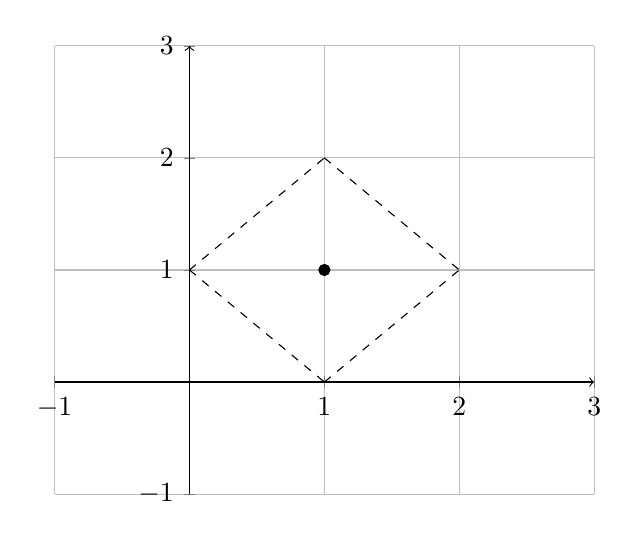
\begin{tikzpicture}
	\begin{axis}[
	axis lines=middle,
	axis line style={->},
	grid=both,
	xmin=-1, xmax=3,
	ymin=-1, ymax=3,
	xtick={-1,...,3}, ytick={-1,...,3}
	]
	\addplot [only marks] table {
		1 1
	};
	
	\addplot [domain=1:2, samples=2, dashed] {-1*x+3};
	\addplot [domain=0:1, samples=2, dashed] {-1*x+1};
	\addplot [domain=0:1, samples=2, dashed] {1*x+1};
	\addplot [domain=1:2, samples=2, dashed] {1*x-1};
	
	\end{axis}
	\end{tikzpicture}
\end{figure}

\subsection{Prüfungs SS17}

\subsubsection{Aufgabe 1}

Aufgabe a:


\begin{figure}[h]
	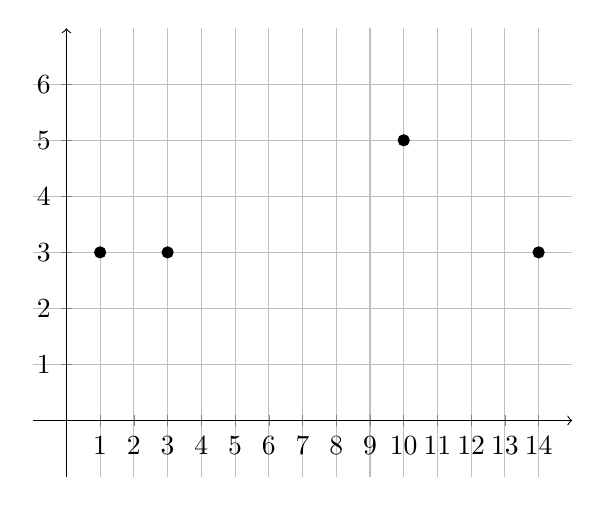
\begin{tikzpicture}
	\begin{axis}[
	axis lines=middle,
	axis line style={->},
	grid=both,
	xmin=-1, xmax=15,
	ymin=-1, ymax=7,
	xtick={0,...,14}, ytick={0,...,6}
	]
	\addplot [only marks] table {
		1 3
		3  3
		10  5   
		14  3
	};
	
	%\ [domain=-10:16, samples=2, dashed] {-0.48*x+6.86};
	\end{axis}
	\end{tikzpicture}
\end{figure}
Aufgabe b:\\	
	$\mu_{1} = 
	\begin{pmatrix}
		2\\
		3
	\end{pmatrix}$
		$\mu_{2} = 
	\begin{pmatrix}
	12\\
	4
	\end{pmatrix}$
	\\
	$S_w = 
		\begin{pmatrix}
		10 & -4\\
		-4 & 1
		\end{pmatrix}
	$
	\\
	$w^* = 
		\begin{pmatrix}
			6\\
			12 \frac{1}{2}
		\end{pmatrix}
	$
	$w_{0} = 85.75$
	
\begin{figure}[h]
	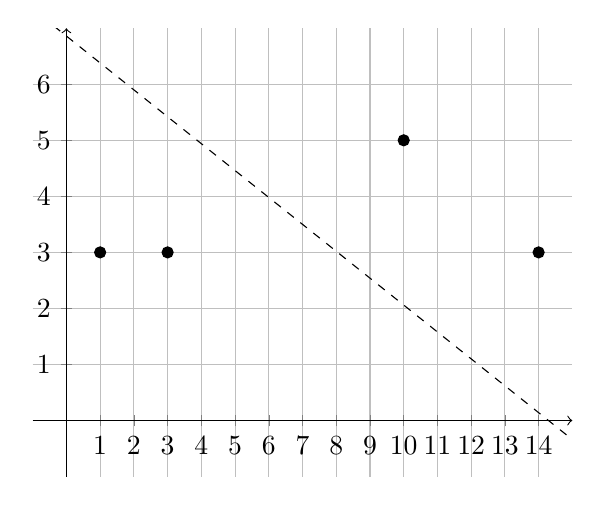
\begin{tikzpicture}
	\begin{axis}[
	axis lines=middle,
	axis line style={->},
	grid=both,
	xmin=-1, xmax=15,
	ymin=-1, ymax=7,
	xtick={0,...,14}, ytick={0,...,6}
	]
	\addplot [only marks] table {
		1 3
		3  3
		10  5   
		14  3
	};
	
	\addplot [domain=-10:16, samples=2, dashed] {-0.48*x+6.86};
	\end{axis}
	\end{tikzpicture}
\end{figure}

Aufgabe c:


\end{document}
